%-----------------------------------LICENSE------------------------------------%
%   This file is part of tikz_figures.                                         %
%                                                                              %
%   tikz_figures is free software: you can redistribute it and/or              %
%   modify it it under the terms of the GNU General Public License as          %
%   published by the Free Software Foundation, either version 3 of the         %
%   License, or (at your option) any later version.                            %
%                                                                              %
%   tikz_figures is distributed in the hope that it will be useful,            %
%   but WITHOUT ANY WARRANTY; without even the implied warranty of             %
%   MERCHANTABILITY or FITNESS FOR A PARTICULAR PURPOSE.  See the              %
%   GNU General Public License for more details.                               %
%                                                                              %
%   You should have received a copy of the GNU General Public License along    %
%   with tikz_figures.  If not, see <https://www.gnu.org/licenses/>.           %
%------------------------------------------------------------------------------%

% Use the standalone class for displaying the tikz image on a small PDF.
\documentclass[crop, tikz]{standalone}

% Import the tikz package to use for the drawing.
\usepackage{tikz}

% Needed for blackboard bold C.
\usepackage{amssymb}

% The arrow package is used for the LaTeX arrow.
\usetikzlibrary{arrows.meta}

% Begin the document.
\begin{document}

    % Draw the figure.
    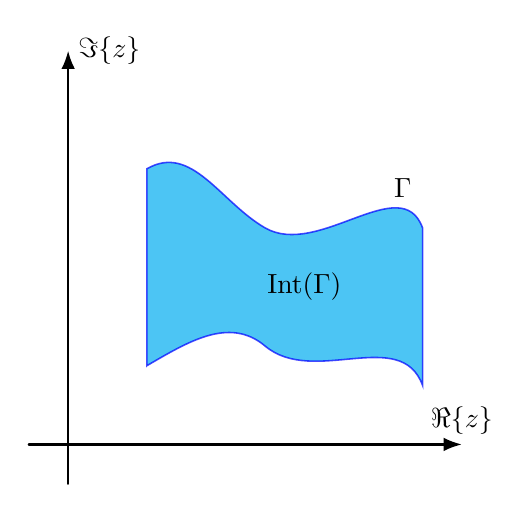
\begin{tikzpicture}[%
        > = Latex,
        line width = 0.2mm,
        line cap = round,
        scale = 2.5
    ]

        % coordinates for the points that define the Jordan curve.
        \coordinate (P1) at (0.4, 0.4);
        \coordinate (P2) at (0.4, 1.4);
        \coordinate (P3) at (1, 1.1);
        \coordinate (P4) at (1.8, 1.1);
        \coordinate (P5) at (1.8, 0.3);
        \coordinate (P6) at (1, 0.5);

        % Axes.
        \begin{scope}[thick]
            \draw[->] (-0.2, 0) to (2, 0) node [above] {$\Re\{z\}$};
            \draw[->] (0, -0.2) to (0, 2) node [right] {$\Im\{z\}$};
        \end{scope}

        % Draw the Jordan curve and color the interior cyan.
        \draw[blue, fill = cyan, opacity = 0.7]
            (P1) to
            (P2) to [out = 30, in = 150]
            (P3) to [out = -30, in = 110]
            (P4) to       
            (P5) to [out = 110, in = -40]
            (P6) to [out = 140, in = 30] cycle;

        % Labels for the Jordan curve and its interior.
        \node at (1.2,0.8) {$\textrm{Int}(\Gamma)$};
        \node at (1.7,1.3) {$\Gamma$};
    \end{tikzpicture}
\end{document}
